\documentclass[12pt]{article}
\usepackage[utf8]{inputenc}
\usepackage[english,russian]{babel}
\usepackage[left=2cm,top=2cm,right=2cm,bottom=2cm]{geometry}
\usepackage{enumitem}
\usepackage{amssymb}
\usepackage[pdftex]{graphicx}
\setlist{nolistsep, parsep=3pt}

\begin{document}
	
	\begin{center}
		{\large{\bf Алгоритм Форда-Фалкерсона нахождения максимального потока\newline в транспортной сети}}
	\end{center}
	~\\
	
	\begin{flushright}
		\parВыполнил: Рычков А.Е.
		\parСтудент 332 группы
	\end{flushright}
	~\\
	~\\
	{\large{\bfВведение}}
	~\\
	\par Ориентированный граф можно интерпретировать как некоторую транспортную сеть и использовать для решения задач о потоках вещества в системе трубопроводов. Каждое ориентированное ребро сети можно рассматривать как канал, по которому движется продукт. Каждый канал имеет заданную пропускную способность, которая характеризует максимальную скорость перемещения продукта по каналу. Вершины являются точками пересечения каналов, через вершины, отличные от истока и стока, продукт проходит, не накапливаясь. Иными словами, скорость поступления продукта в вершину должна быть равна скорости его удаления оттуда.
	~\\
	~\\
	{\large{\bfОсновные понятия}}
	~\\
	\par {\bfТранспортная сеть} (flow network) $G = (V, E)$ представляет собой ориентированный граф, в котором каждое ребро $(u, v) \in E$ имеет неотрицательную пропускную способность (capacity) $c(u,v) \ge 0$.В случае, если $E$ содержит ребро $(u, v)$, обратного ребра $(v, u)$ быть не должно. Если $(u,v)\notin E$, то $c(u,v)=0$, петли также запрещены. Также выделяются две вершины: исток (source) s и сток (sink) t. Каждая вершнина лежит на некотором пути от истока к стоку, то есть для любой вершины $v \in V$ транспортная сеть содержит путь $s \rightarrow v \rightarrow t$. Таким образом, граф является связным, следовательно каждая вершина, отличная от s, содержит как минимум одно входящее ребро ( $|E| \ge |V| - 1$ ).
	\par{\bfПотоком}(flow) является действительная функция $f : V \rightarrow \mathbb{R}$, удовлетворяющая следующим условиям:\newline
	Ограничение пропускной способности. Для всех $u, v \in V$ должно выполняться $0 \le f(u,v) \le c(u,v)$.\newline
	Сохранение потока. Для всех $u \in V - \{s, t\}$ должно выполняться
	$$ \sum_{v \in V}{f(u,v)} = \sum_{v \in V}{f(v,u)} $$
	Когда $(u, v) \notin E$, потока из u в v быть не может, так что $f(u,v) = 0$.
	\par{\bfВеличина потока} $|f|$ потока $f$ определяется как
	$$ |f| = \sum_{v \in V}{f(s,v)} - \sum_{v \in V}{f(v,s)} $$
	\newpage
	\par {\bfОстаточную пропускную способность}  $c_f(u,v)$ введем как
	$$ c_f(u,v) =  
	\left\{
		\begin{array}{rcl}
		c(u,v) - f(u,v), & \mbox{если} \; (u,v) \in E, \\
		f(v,u), & \mbox{если} \; (v,u) \in E, \\
		0 & \;\;\; \mbox{в противном случае.}
		\end{array}
	\right.  $$
	\par{\bfОстаточная сеть} для $G = (V, E)$ и потока $f$ представляет собой граф $G_f = (V, E_f)$, где
	$$ E_f = \{(u,v) \in V \times V : c_f(u,v) > 0\}$$\newline
	Ребра в $E_f$ являются либо ребрами из $E$, либо обратные им, таким образом, $|E_f| \le 2|E|$. Остаточная сеть удовлетворяет всем свойствам транспортной сети, кроме того, что она может содержать одновременно и ребро $(u,v)$, и $(v, u)$.
	\par{\bfУвеличение потока} $f$ в транспортной сети $G$ на $f'$ из остаточной сети  $G_f$ определяется как функция, отображающая $V \times V \mbox{на } \mathbb{R}$:
	$$ (f \uparrow f)(u,v) =
	\left\{
		\begin{array}{rcl}
			f(u,v) + f'(u,v) - f'(v,u), & \mbox{если} \; (u,v) \in E, \\
			0 & \mbox{в противном случае}
		\end{array}
	 \right. $$
	 \par {\bfЛемма об увеличении потока}
	 \par (Здесь и далее леммы и теоремы приводятся без доказательств)
	 \par Пусть $G = (V, E)$ является транспортной сетью с истоком $s$ и стоком $t$ и пусть $f$ представляет собой поток в $G$. Пусть $G_f$ - остаточная сеть $G$, порожденная $f$, и пусть $f'$ - поток в $G_f$. Тогда функция $f \uparrow f'$ представляет собой поток в $G$ с величиной $|f \uparrow f'| = |f| + |f'|$.
	\par{\bfУвеличивающим путем} $p$ для транспортной сети $G = (V, E)$ и потока $f$ является простой путь из $s$ в $t$ в остаточной сети $G_f$.
	\par{\bfОстаточная пропускная способность} -  это максимальная величина, на которую можно увеличить поток в каждом ребре увеличивающего пути $p$, и которая задается формулой
	$$c_f(p) = min\{c_f(u,v) : (u,v) \in p\}$$
	\par{\bfЛемма об остаточной пропускной способности}
	\par Пусть $G = (V, E)$ является транспортной сетью, а $f$ представляет собой поток в $G$, и пусть $p$ является увеличивающим путем в $G_f$. Определим функцию $f_p : V \times V \rightarrow \mathbb{R}$ как
	$$ f_p(u,v) =
	\left\{
		\begin{array}{rcl}
			c_f(p), & \mbox{если} \; (u,v) \in p, \\
			0 & \mbox{в противном случае}
		\end{array}
	 \right. $$ 
	Тогда $f_p$ является потоком в $G_f$ с величиной $|f_p| = c_f(p) > 0$.
	\par{\bfСледствие}
	\par Пусть $G = (V, E)$ представляет собой транспортную сеть, а $f$ является потоком в $G$ , и пусть $p$ представляет собой увеличивающий путь в $G_f$. Пусть также $f_p$ определен, как в предыдущем уравнении, и предположим, что мы увеличиваем $f$ на $f_p$. Тогда функция $f \uparrow f_p$ является потоком в $G$ с величиной $|f \uparrow f_p| = |f| + |f_p| > |f|$
	\par{\bfРазрезом} $(S, T)$ транспортной сети $G = (V,E)$ называется разбиение множества вершин $V$ на множества $S$ и $T = V - S$, такие, что $s \in S$, а $t \in T$.
	\par{\bfЧистый поток} $f(S,T)$ через разрез $(S, T)$ определяется как
	$$ f(S,T) = \sum_{u \in S}\sum_{v \in T}f(u,v) - \sum_{u \in S}\sum_{v \in T}f(v,u) $$
	\par{\bfПропускной способностью разреза} $(S,T)$ является
	$$ c(S,T) = \sum_{u \in S}\sum_{v \in T}c(u,v) $$
	\par{\bfМинимальным разрезом} сети является разрез, пропускная способность которого среди всех разрезов сети минимальна.
	\par{\bfЛемма о чистом потоке}
	\par Пусть $f$ представляет собой поток в транспортной сети $G$ со стоком $s$ и истоком $t$ и пусть $(S, T)$ - произвольный разрез $G$. Тогда чистый поток через разрез $(S, T)$ равен $f(S, T) = |f|$.
	\par{\bfСледствие}
	\par Величина любого потока $f$ в транспортной сети $G$ ограничена сверху пропускной способностью произвольного разреза $G$.
	~\\
	~\\
	{\large{\bfТеорема о максимальном потоке и минимальном разрезе}}
	~\\
	\par Если $f$ представляет собой поток в транспортной сети $G = (V, E)$ с истоком $s$ и стоком $t$, то следующие утверждения эквивалентны.
	\begin{enumerate}
		\item $f$ является максимальным потоком в $G$.
		\item Остаточная сеть $G_f$ не содержит увеличивающих путей.
		\item $|f| = c(S,T)$ для некоторого разреза $(S, T)$ транспортной сети $G$.
	\end{enumerate}
	~\\
	~\\
	{\large{\bfФормулировка задачи о максимальном потоке}}
	~\\
	\par Дана некоторая транспортная сеть $G = (V,E)$ с истоком $s$ и стоком $t$, и необходимо найти поток максимальной величины.
	~\\
	~\\
	{\large{\bfАлгоритм Форда-Фалкерсона}}
	~\\
	\begin{enumerate}
		\item {\bfДля} каждого ребра $(u,v) \in G.E$
		\item ~~ $ (u,v).f = 0$
		\item {\bfПока} существует путь $p$ из $s$ в $t$ в остаточной сети $G_f$
		\item ~~ $c_f(p) = min\{c_f(u,v) : (u,v) \in p\}$
		\item ~~ {\bfДля} каждого ребра $(u,v)$ в $p$
		\item ~~~~ {\bfЕсли} $(u,v) \in E$
		\item ~~~~~~ $(u,v).f = (u,v).f + c_f(p)$
		\item ~~~~ {\bfИначе} $(v,u).f = (v,u).f - c_f(p)$
	\end{enumerate}
	~\\
	~\\
	{\large{\bfПримечания к реализации алгоритма}}
	~\\
	\par Алгоритм был реализован мною на языке C. Функция, отвечающая за алгоритм – int findMaxFlow(int n, int c[n][n]). В качестве параметров принимает кол-во вершин и матрицу смежности с значениями пропускной способности для каждого ребра, а возвращает величину максимального потока в сети.
	\par В качестве основной структуры данных был использован двумерный статический массив. Поиск увеличивающего пути в остаточной сети ведется с помощью алгоритма поиска в ширину.
	~\\
	~\\
	{\large{\bfАнализ алгоритма}}
	~\\
	\par Время выполнения алгоритма зависит от того, как именно выполняется поиск увеличивающего пути в строке 3. Если увеличивающий путь выбирается с использованием алгоритма поиска в ширину, то алгоритм выполняется за полиномиальное время. Если значения пропускной способности ребер являются иррациональными числами, то величина потока не будет сходиться к максимальной величине потока. Если пропускные способности являются рациональными числами, то можно использовать соответствующее масштабирование, чтобы сделать их целыми.
	\par Если обозначить максимальный поток в сети как $f^*$, то цикл while выполняется не более $|f^*|$  раз, поскольку величина потока за каждую итерацию увеличивается по крайней мере на единицу.
	\par Цикл будет выполняться наиболее эффективно, если реализовать транспортную сеть $G = (V, E)$ с помощью правильно выбранной структуры данных и искать увеличивающий путь с помощью алгоритма с линейным временем работы. Например, если мы поддерживаем структуру данных, соответствующую ориентированному графу $G' = (V, E')$, где $E' = \{(u,v) \in E \mbox{ или } (v,u) \in E$. Ребра сети $G$ являются также ребрами графа $G'$, поэтому в такой структуре данных можно легко хранить пропусные способности и потоки. Для данного потока $f$ в $G$ ребра остаточной сети $G_f$ состоят из всех ребер $(u,v)$ графа $G'$, таких, что $c_f(u,v) > 0$. Следовательно, время поиска пути в остаточной сети составляет O$(V + E') = \mbox{O}(E)$, если используется поиск в глубину или ширину. Таким образом, итерация цикла while занимает время O$(E)$, что вместе с инициализацией делает общее время выполнения равным О$(E|f^*|)$.
	~\\
	~\\
	{\large{\bfСравнение практической и теоретической части}}
	~\\
	\par Проверим, действительно ли цикл while будет выполняться не более $|f^*|$ раз. Проведем тест при $|V| = 10 : 100$, при этом пропускная способность каждого ребра ( кроме, естественно, петель и обратных ребер) задается случайно в диапазоне $0: 10$. Для каждого $|V|$ повторим 5 раз, затем аппроксимируем результаты, для получения наиболее приближенной к действительности картины зависимости кол-ва итераций от величины максимального потока. На графике ось абсцисс взята за $|f^*|$, а ось ординат за количество итераций.
	\begin{center}
	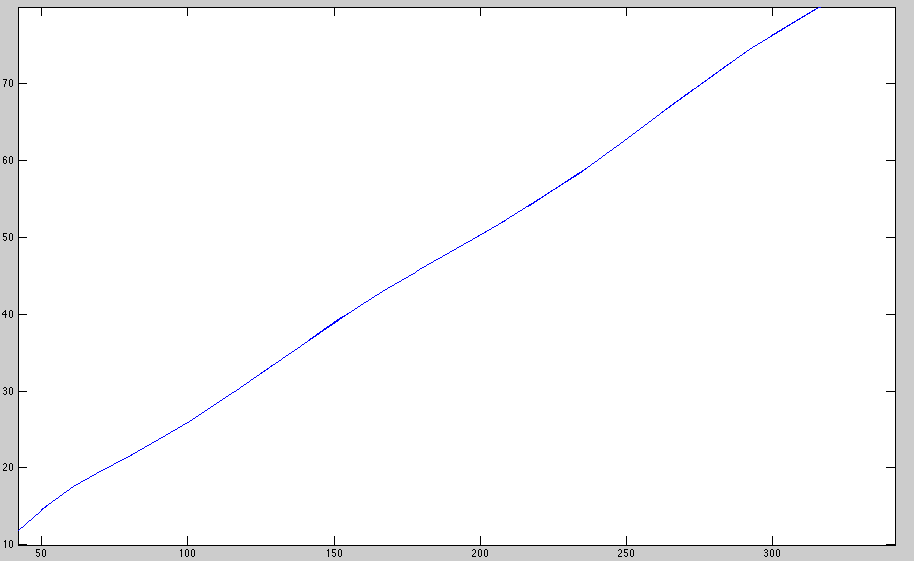
\includegraphics[width=0.9\linewidth]{kF}\newline
	Как видно из графика,теория успешно совпадает с практикой.
	\end{center}
	\par Cледует заметить, что при увеличении пропускной способности такая зависимость по-прежнему будет соблюдаться, при этом увеличится величина добавляемого потока.
	\par Далее проиллюстрируем влияние рамера задачи на время выполнения алгоритма. Проведем указанные выше операции, но при этом засечем время нахождения ( в миллисекундах ) каждого максимального потока.
	\begin{center}
	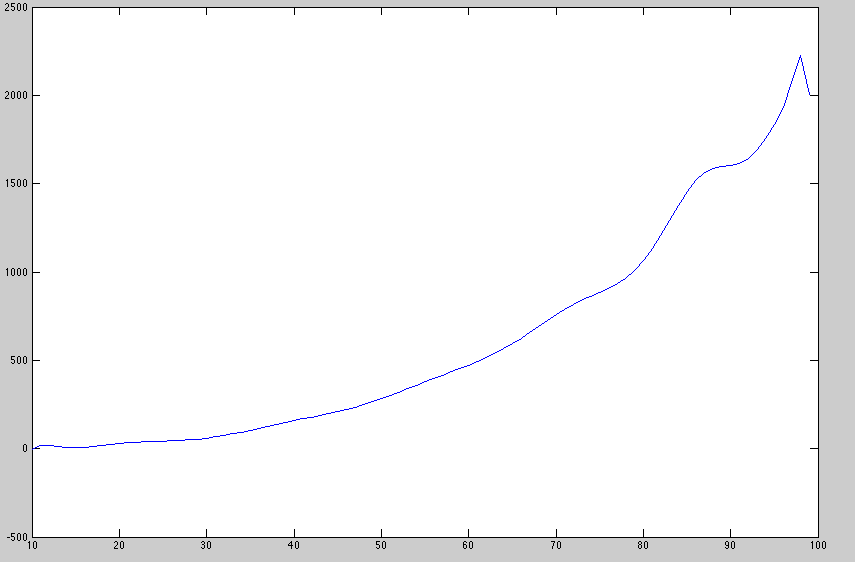
\includegraphics[width=0.9\linewidth]{NT}
	\end{center}
	\par А также покажем зависимость кол-ва элементарных операций от размера входных данных.
	\begin{center}
	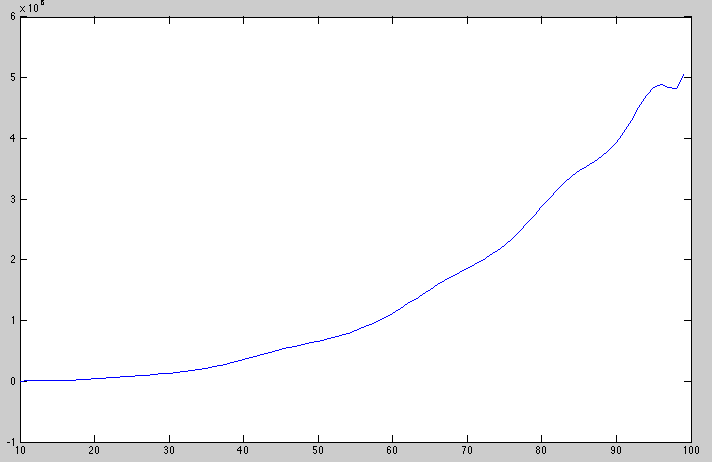
\includegraphics[width=0.9\linewidth]{NO}
	\end{center}
	\par Алгоритм выполняет намного больше элементарных операций, чем указано в его теоретической сложности. Но это обусловлено конкретной реализаций, если считать только те элементарные операции, которые обговорены в псевдокоде, то теоретическая сложность действительно будет выполняться.
	~\\
	~\\
	{\large{\bfВывод}}
	~\\
	\par Классический алгоритм поиска максимального потока. Но далеко не самый лучший (если быть более точным, второй с конца по сложности). Хорош для обучения, но в целях практического применения стоит воспользоваться его модификациями или более быстрыми алгоритмами.
	~\\
	~\\
	{\large{\bfЛитература}
	~\\
	\begin{enumerate}
		\item Томас Кормен, Чарльз Лейзерсон, Рональд Ривест, Клиффорд Штайн\newline "Алгоритмы. Построение и анализ."
		\item https://ru.wikipedia.org/
		\item http://algolist.manual.ru/maths/graphs/maxflows/
		\item http://informatics.mccme.ru/mod/book/view.php?id=448
	\end{enumerate}
	
	
\end{document}